\section{Prüfung der Vollständigkeit}

Von \cite{shanbhag2014optimizing} wurde die Vollständigkeit der Regelmenegen geprüft. Eine Regelmenge wird dann als vollständig gewertet, wenn sie genutzt werden kann, um einen Suchraum von allen kreuzproduktfreien Plänen aus einem initialen Plan, der keine Kreuzprodukte enthält, zu erzeugen. In diesem Zusammenhang lassen sich drei Aspekte genauer betrachteten: (1) alle Pläne müssen gefunden werden; (2) die Pläne müssen kreuzproduktfrei sein; (3) sie müssen aus einem initialen Plan ohne Kreuzprodukte gebildet werden.

Um sicherzustellen, dass die erzeugten Pläne kreuproduktfrei sind, wurde von \cite{shanbhag2014optimizing} ein Mechanismus zur Kreuzproduktunterdrückung implementiert. Der Mechanismus sieht vor, dass nachdem ein neuer Plan mit Hilfe einer Regel erzeugt wurde, geprüft wird ob der erzeugte Plan kreuzproduktfrei ist. Nur wenn das der Fall ist wird der neue Plan gespeichert. Falls der neue Plan Kreuzprodukte enthält, wird die Regel zwar als ausgeführt markiert, aber das Ergebnis nicht gespeichert. Nur Ergebnisse, die kreuzproduktfrei sind, werden als Input für eine Regel akzeptiert. Regelmengen, die Kreuzprodukte durch diesen Mechnanismus verhindern,  werden mit dem Postfix -CPS versehen. So entstehen die neuen Regelmengen RS-B0-CPS, RS-B1-CPS und RS-B2-CPS.






\subsection{Prüfung von Regelmenge RS-B0-CPS und RS-B1-CPS}

Bei der Prüfung der beiden Regelmengen RS-B0-CPS und RS-B1-CPS auf Vollständigkeit wurde zuerst festgestellt, dass wenn RS-B1-CPS vollständig ist auch automatisch RS-B0-CPS als vollständig gilt. Dies lässt sich darauf zurückführen, dass im Gegensatz zu RS-B1-CPS die Regelmenge RS-B0-CPS eine weitere, zusätzliche Regel implementiert. Da bereits die Regelmenge RS-B1-CPS vollständig ist, ist auch automatisch die Regel RS-B0-CPS vollständig, da die zusätzliche Regel keine bisher unbekannten Pläne erzeugen kann.

In einem ersten Schritt wird gezeigt, dass für jeden Join-Graphen ein kreuzprodukfreier links-tiefer Baum erzeugt werden kann. 
Aus einem gegebenenen Join-Graphen $G = (V, E)$ kann ein links-tiefer Baum gebildet werden, indem ein belibiger Knoten $v \in V$ als Start-Teilbaum $T_1$ gewählt wird. Aus dem $G$ wird dann ein beliebiger Knoten ausgewählt, der mit einem Knoten aus $T_i$ über eine Kante $e \in E$ verbunden ist, aber nicht Teil von $T_i$. Dieser Knoten wird dann mit dem Teilbaum $T_i$ verknüpft, so dass ein neuer Teilbaum entsteht. Sobald alle Knoten $V$ Teil des Teilbaums sind, ist ein kreuzproduktfreier Baum gebildet.

\newtheorem{lem}{Lemma} 

\begin{Lemma}
Gegeben sei ein kreuzproduktfreier Baum mit den Relationen $R_1, R_2, ... R_k$. Es ist möglich diesen Baum in einen Baum $T \Join R_k$ mit RS-B1-CPS zu transformieren, wobei $T$ ein Join-Tree estehend aus $R_1, R_2, ..., R_k-1$ ist.

\end{Lemma}










Es wurde angenommen, dass für einen kreuzproduktfreien Baum mit den Relationen $R_1, R_2, ..., R_k$


\subsection{Unvollständigkeit von RS-B2}

\begin{figure}[ht]
  \centering
  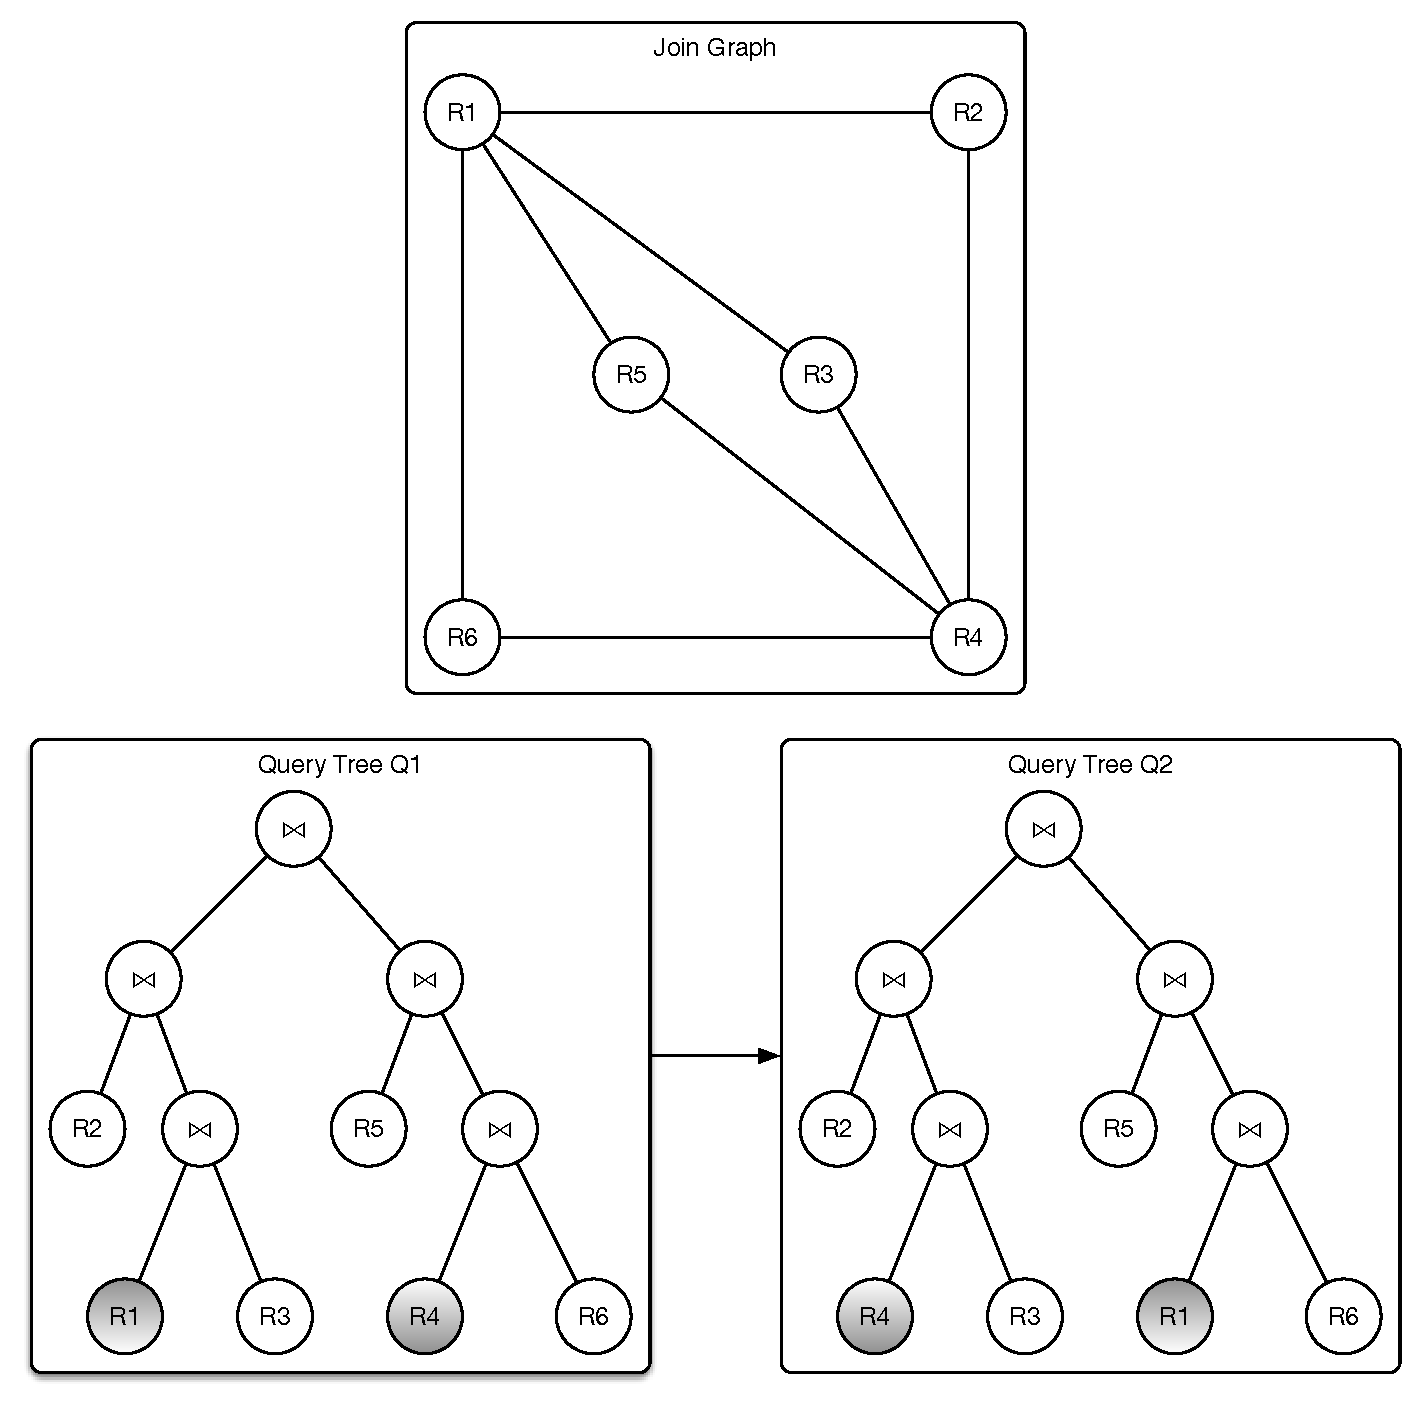
\includegraphics[width=\textwidth]{02_Related_Work/Graphs.pdf}
  \caption{Incompletness of RS-B2-CPS}
  \label{Incompleteness_RS-B2-CPS}
\end{figure}


Die Unvollständigkeit wurde mit Hilfe eines Beispiels belegt. Als Beispiel wurde der Bushy-Tree gewählt, der in Abbildung \ref{Incompleteness_RS-B2-CPS} zu sehen ist. Mit Hilfe der Regeln aus der Regelmenge RS-B2 sollte der initale Plan () in den Plan () umgewandelt werden. Dabei werden die vier Regeln der Regelmenge angewendet.

\begin{itemize}
\item Mit der Kommutativitätsregel ist es möglich ein Spiegelbild des original Baums herzustellen, aber nicht den Plan grundlegend zu verändern.
\item Bei der Anwendung von linker Assoziativität auf den Root-Knoten des Baum würde ein neuer Baum erzeugt werden dessen
\item Das Ergebnis von rechter Assoziativität ist symmetrisch zu linker Assoziativität.
\end{itemize}


Welche Regel auch immer auf den Baum angewendet wird, es ist nicht möglich den einen in den anderen Baum zu transformieren.

\subsection{Unvollständigkeit von RS-B2 mit Hilfe von PyroJ}

Mit Hilfe des Optimierers PyroJ - sein Aufbau wird in \ref{sec:pyroJ} behandelt - wurden die Regelsets ebenfalls auf ihre Vollständigkeit hin geprüft. Es wurde angenommen, dass zwei Ergebnismengen dann gleich sind, wenn die Anzahl der Äquivalenzklassen und die Anzahl der Operatorknoten gleich ist. Da wie zuvor festgestellt RS-B1 vollständig ist, wurde RS-B1 als Benchmark für andere Regelsets genutzt. Als Test-Case wurden Starqueries verwendet. Wie in Tabelle \ref{} zu sehen ist, wurde mit Hilfe von RS-B2 erheblich weniger Operatoren-Knoten erzeugt als mit RS-B1. \cite{} schlisst daher darauf, dass RS-B2 unvollständig ist.

Ebenfalls stellt \cite{} hervor, dass eine bestimmte Anfrage (Anfrage 7 des TPC-DS Benchmarks) bei der Nutzung des RS-B2 eine um 1.86 höher geschätzte Kosten als RS-B1 verursacht hatte.

